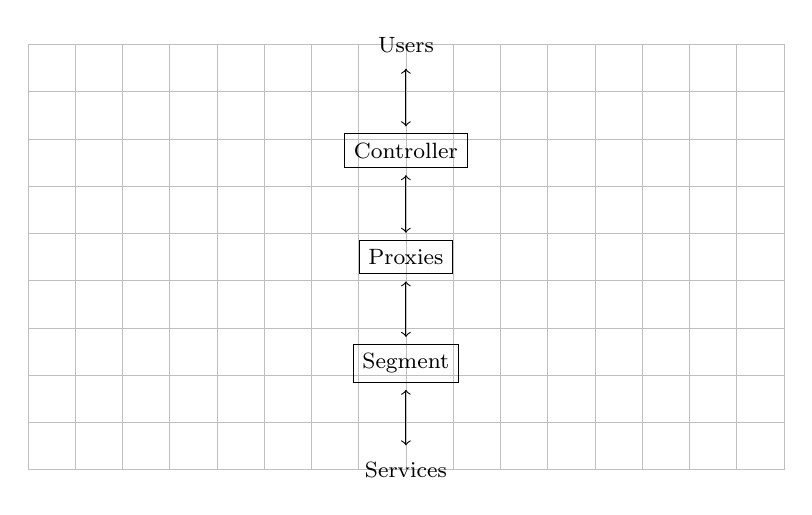
\begin{tikzpicture}[
	scale = 0.6,
	rect/.style={
		rectangle,
		draw=black
	},
	circ/.style={
		circle,
		draw=black
	},
	every node/.style={
		font=\footnotesize
	}
]{
		\def\width{16}
		\def\height{9}
		\draw[help lines, opacity=0.5] (0,0) grid (\width,\height);
		\node(p1) at (8,9){Users};
		\node(c1)[rect] at (8,6.75){Controller};
		\node(pr1)[rect] at (8,4.5){Proxies};
		\node(s1)[rect] at (8,2.25){Segment};
		\node(p2) at (8,0){Services};
		
		\path[<->, shorten >= 0.25em, shorten <= 0.25em] (p1.south) edge (c1.north);
		\path[<->, shorten >= 0.25em, shorten <= 0.25em] (c1.south) edge (pr1.north);
		\path[<->, shorten >= 0.25em, shorten <= 0.25em] (pr1.south) edge (s1.north);
		\path[<->, shorten >= 0.25em, shorten <= 0.25em] (s1.south) edge (p2.north);
}
\end{tikzpicture}